\documentclass[letterpaper]{article}
\usepackage[submission]{aaai2027}
\usepackage[hyphens]{url}
\usepackage{graphicx}
\graphicspath{{figures/}{paper_v4/figures/}}
\urlstyle{rm}
\def\UrlFont{\rm}
\usepackage{natbib}
\usepackage{caption}
\frenchspacing
\usepackage{amsmath}
\usepackage{booktabs}
\pdfinfo{
/TemplateVersion (2027.1)
}

\setcounter{secnumdepth}{1}

\title{Supplementary Material}
\author{Parsuram Pradhan}
\affiliations{}

\begin{document}

\maketitle

\noindent Supplement to \emph{Cost-Aware Reinforcement Learning for Agentic RAG}. The main paper states every result its claims use. This note records the reward presets, the observation vector, the training curves and the extrapolated hours, the prompts, the Adaptive-RAG validation grid, two example trajectories, and the corpus counts.

\section{Reward Weights and the Price Card}
Table~\ref{tab:presets} is every preset in \texttt{configs/reward\_weights.yaml}. The frozen rows use \texttt{default}. The rewrite-first exam uses \texttt{frontier\_lambda20}. The retrieve-first sweep uses \texttt{frontier\_lambda0}, \texttt{frontier\_lambda5}, \texttt{frontier\_lambda20}, and \texttt{frontier\_lambda80}, with the action charge at 0. \texttt{frontier\_act02} is the older \(\lambda{=}80\) preset and keeps the charge at 0.02. The unused-budget bonus is paid only when \(Q_{\mathrm{ans}}\) clears the quality gate.

\begin{table*}[t]
\centering
\small
\begin{tabular}{lcccccccccc}
\toprule
Preset & \(\alpha\) & \(\beta\) & \(\gamma\) & \(\lambda\) & \(\mu\) & Hall. & \(\rho\) & Budget & Gate & Bonus \\
\midrule
default & 1 & 0.4 & 0.15 & 2 & 0.5 & 0.5 & 0.02 & 1 & 0.5 & 0.1 \\
correctness\_only & 1 & 0 & 0 & 0 & 0 & 0 & 0 & 0 & 0 & 0 \\
correctness\_grounding & 1 & 0.4 & 0 & 0 & 0 & 0.5 & 0 & 0 & 0 & 0 \\
correctness\_faithfulness\_cost & 1 & 0.4 & 0 & 2 & 0.5 & 0.5 & 0.02 & 1 & 0.5 & 0.1 \\
lambda\_zero & 1 & 0.4 & 0.15 & 0 & 0 & 0.5 & 0.02 & 1 & 0.5 & 0.1 \\
high\_cost\_pressure & 1 & 0.4 & 0.2 & 8 & 2 & 0.5 & 0.05 & 1 & 0.5 & 0.2 \\
frontier\_lambda0 & 1 & 0.4 & 0.15 & 0 & 0.5 & 0.5 & 0 & 1 & 0.5 & 0.1 \\
frontier\_lambda5 & 1 & 0.4 & 0.15 & 5 & 0.5 & 0.5 & 0 & 1 & 0.5 & 0.1 \\
frontier\_lambda20 & 1 & 0.4 & 0.15 & 20 & 0.5 & 0.5 & 0 & 1 & 0.5 & 0.1 \\
frontier\_lambda80 & 1 & 0.4 & 0.15 & 80 & 0.5 & 0.5 & 0 & 1 & 0.5 & 0.1 \\
frontier\_act02 & 1 & 0.4 & 0.15 & 80 & 0.5 & 0.5 & 0.02 & 1 & 0.5 & 0.1 \\
\bottomrule
\end{tabular}
\caption{Reward presets. Hall.\ is the hallucination weight. \(\rho\) is the per-action charge after the first action. Budget is the unit penalty for a hard-budget break. Gate is the \(Q_{\mathrm{ans}}\) threshold for the unused-budget bonus.}
\label{tab:presets}
\end{table*}

The price card meters local tokens at \$0.15 per million input tokens and \$0.60 per million output tokens. BM25 is \(5\times 10^{-5}\) dollars per call. The latency term uses a fixed table, not the wall clock: 212.4 ms per retrieve, 999.2 ms per rewrite, 143.2 ms per rerank, 0 ms per verify, and 853.9 ms plus 52.0 ms per completion token for a generation. The latency weight is 0.5 and the unit is \(10^{-3}\) dollars per second. Logged latency remains the measured time.

\FloatBarrier
\section{Observation}
The rewrite-first policy reads 16 numbers. There is no question text, no dataset indicator, and no passage text. Before any retrieval the four score channels are 0. The retrieve-first controller appends nine numbers after these sixteen: question length, who, what, when, which, a yes/no bit, a capitalized-entity count, draft abstention, and draft overlap with the top passage.
\begin{enumerate}
\item Mean of the top-five BM25 scores, z-scored on the training slice and clipped to \([-3, 3]\).
\item Evidence count, divided by 10 and clipped to 1.
\item Remaining steps, divided by the step cap.
\item Remaining budget, divided by the dollar cap and clipped to \([0, 1]\).
\item Verifier support, else 0.
\item Verifier contradiction, else 0.
\item Retrieve count, divided by 3 and clipped to 1.
\item Rewrite count, divided by 2 and clipped to 1.
\item Rerank count, divided by 2 and clipped to 1.
\item Verify count, divided by 2 and clipped to 1.
\item Top-1 BM25 score, z-scored and clipped to \([-3, 3]\).
\item Gap between the top two BM25 scores, z-scored and clipped to \([-3, 3]\).
\item Verify one-hot, support.
\item Verify one-hot, contradiction.
\item Verify one-hot, neutral.
\item Minimum of the top-five BM25 scores, z-scored and clipped to \([-3, 3]\).
\end{enumerate}

\FloatBarrier
\section{Training}
Both networks are one hidden layer of width 16. The rewrite-first network reads 16 numbers and has 357 parameters. The retrieve-first network reads 25 numbers and has 501 parameters. The optimizer is Adam. The learning rate is 0.003. Training runs for 20 epochs on 500 questions. The entropy bonus coefficient is 0.01. The advantage on a training question is that question's sampled reward minus the reward of one-shot retrieval on the same question. After each epoch the mode is rolled out on the 180. The checkpoint is the first epoch with the highest greedy reward on that 180. The generator is Qwen2.5-3B-Instruct at temperature 0. Training used one NVIDIA T4.

The rewrite-first seeds 42, 43, and 44 select epochs 17, 14, and 11. Table~\ref{tab:learned} is that exam. The three rows tie on every reported value except the selected epoch. Figure~\ref{fig:curves} is those three curves. The marker is the selected epoch.

The seven retrieve-first runs use the 501-parameter network. At \(\lambda{=}20\), seeds 42, 43, and 44 select epochs 17, 2, and 19. Seed 42 at \(\lambda{=}0\), 5, and 80 selects epochs 18, 7, and 4. The masked seed 45 at \(\lambda{=}20\) selects epoch 12. The \(\lambda{=}20\) seed-42 training is the sweep row, not a second run. Figure~\ref{fig:rfcurves} is those seven curves. The marker is the selected epoch.

The hours are a budget extrapolated from measured step time, not a wall-clock log of the Colab job. For the rewrite-first \(\lambda{=}20\) exam that budget is 11.8 hours for one seed and 35.4 hours for three seeds. For each retrieve-first run the same extrapolation uses that exam's measured milliseconds per step, the run's mean train and validation step counts, and one pass over the 300. It is 9.6, 7.1, and 9.7 hours for \(\lambda{=}20\) seeds 42, 43, and 44, 10.8, 7.9, and 7.1 hours for seed 42 at \(\lambda{=}0\), 5, and 80, and 6.9 hours for the masked seed 45.

\begin{table}[t]
\centering
\small
\setlength{\tabcolsep}{3pt}
\begin{tabular}{ccccccc}
\toprule
Seed & Epoch & HotpotQA & NQ & Correct & Steps & \$ \(\times 10^{-4}\) \\
\midrule
42 & 17 & 52/150 & 48/150 & 100/300 & 4 & 2.02 \\
43 & 14 & 52/150 & 48/150 & 100/300 & 4 & 2.02 \\
44 & 11 & 52/150 & 48/150 & 100/300 & 4 & 2.02 \\
\bottomrule
\end{tabular}
\caption{The three rewrite-first \(\lambda{=}20\) exams. Each seed emits one action string, rewrite then rewrite then retrieve then stop. The rows tie on every reported value except the selected epoch, so no cell is marked as best. One-shot retrieval on the same index scores 100/300 at \(1.72\times 10^{-4}\) dollars. We report the three rows, not a mean.}
\label{tab:learned}
\end{table}

\begin{figure}[t]
\centering
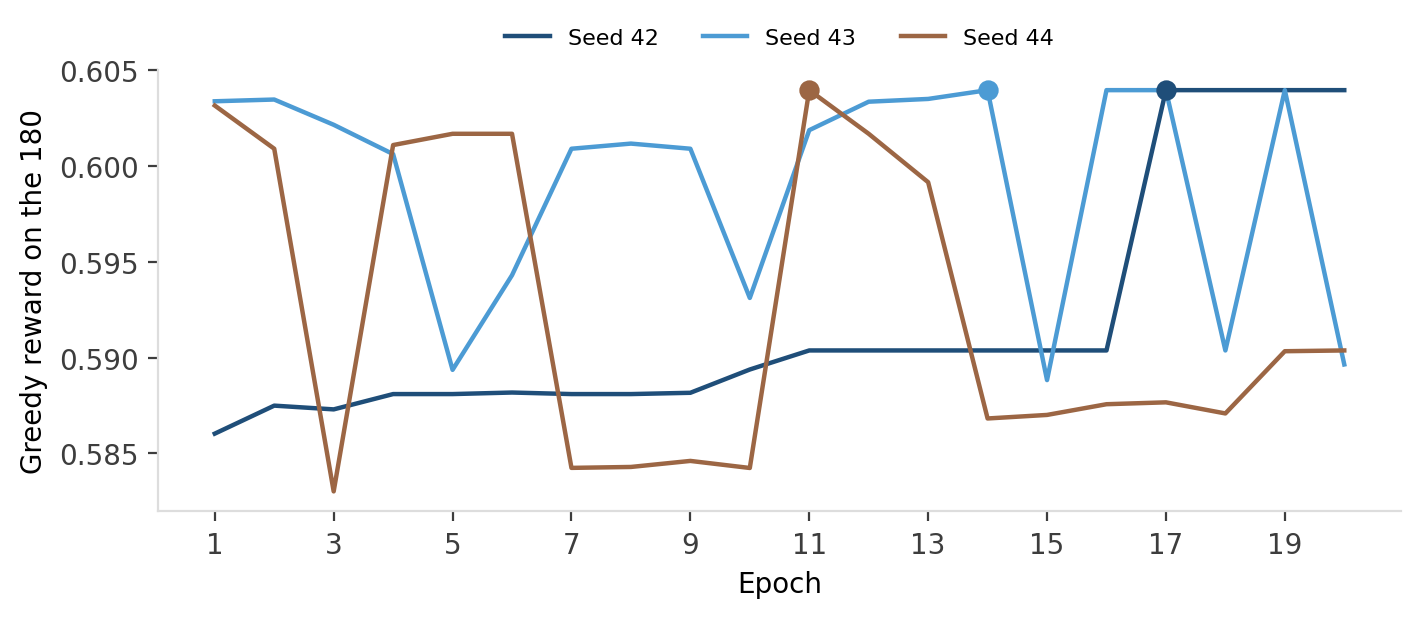
\includegraphics[width=\columnwidth]{train_curves.png}
\caption{Greedy reward on the 180 for the three rewrite-first \(\lambda{=}20\) seeds. The marker is the first epoch of the maximum.}
\label{fig:curves}
\end{figure}

\begin{figure}[t]
\centering
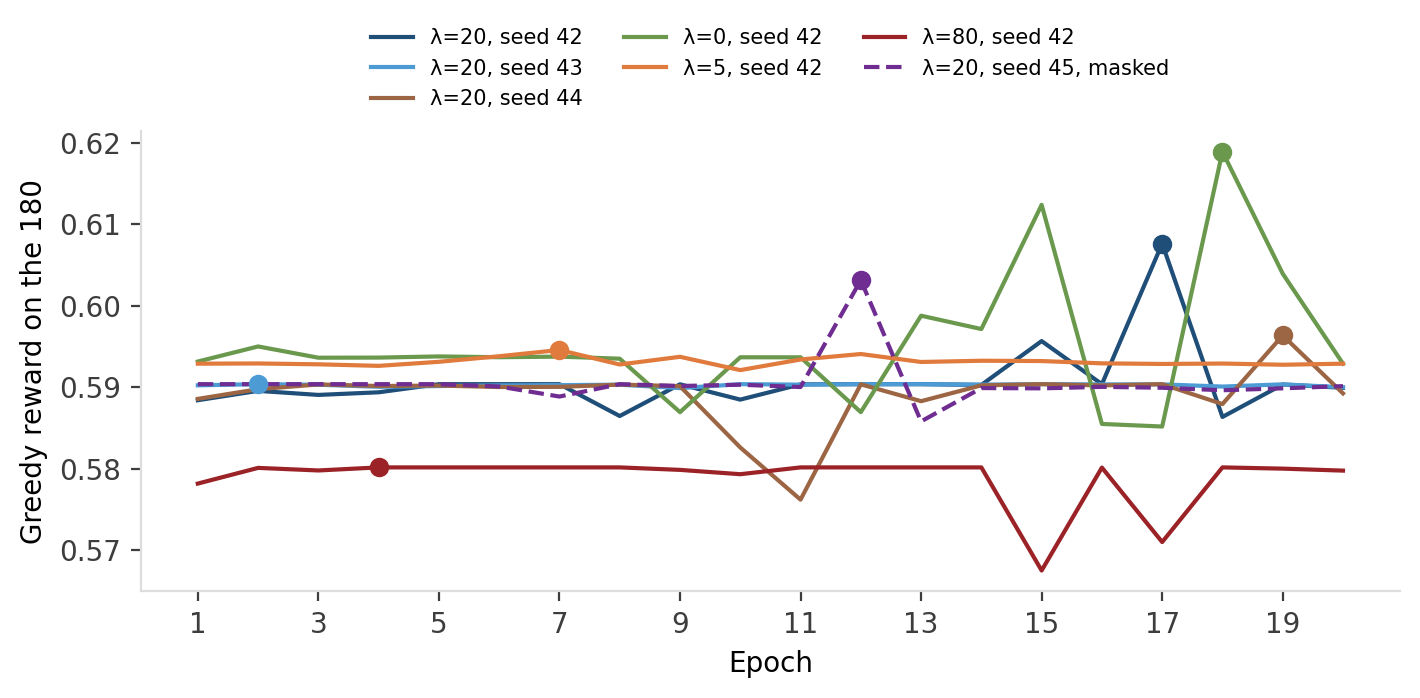
\includegraphics[width=\columnwidth]{train_curves_retrieve_first.png}
\caption{Greedy reward on the 180 for the seven retrieve-first runs. The marker is the first epoch of the maximum. The \(\lambda{=}20\) seed-42 curve is the sweep's \(\lambda{=}20\) row. Seed 45 is the masked controller, and its marker is epoch 12.}
\label{fig:rfcurves}
\end{figure}

\FloatBarrier
\section{Prompts}
Rewrite, system: ``You rewrite search queries for retrieval. Return only the rewritten query, no quotes or explanation.'' User: the original question, the current evidence or ``(no evidence)'', then ``Rewritten query:''.

Yes/no questions, system: ``You are a concise open-domain QA assistant. This is a yes/no question. Reply with exactly yes or no. Do not reply ABSTAIN. Do not explain or quote. Use only the evidence. If the passages name the entities in the question, compare them and answer.''

Other questions, when abstention is allowed, system: ``You are a concise open-domain QA assistant. Answer using only the provided evidence. Reply with a short answer span (a few words when possible). Reply with a short answer span. Never append ABSTAIN after an answer. Use the single token ABSTAIN only if none of the passages could support any answer (empty evidence, or passages about clearly unrelated entities). If a passage title or span could be the answer, you must answer it. Do not use ABSTAIN as a hedge when you are unsure. No explanation and no quotes.'' The user message is the evidence, the question, and ``Answer:''.

\FloatBarrier
\section{Adaptive-RAG Grid}
Table~\ref{tab:grid} is exact match on the 180 for each inverse regularization strength. The test set is not used. Under the first labeling, strengths 10 and 100 tie at 62/180 and strength 100 has the lower mean dollar cost. Under the cheap labeling, every strength sends all 180 questions to one-shot retrieval and scores 58/180, the one-shot total.

\begin{table}[t]
\centering
\small
\begin{tabular}{lcc}
\toprule
Strength & Miss \(\to\) rewrite & Miss \(\to\) one-shot \\
\midrule
0.01 & 59/180 & 58/180 \\
0.1 & 59/180 & 58/180 \\
1 & 59/180 & 58/180 \\
10 & 62/180 & 58/180 \\
100 & 62/180 & 58/180 \\
\bottomrule
\end{tabular}
\caption{Validation exact match for the two labelings. One-shot retrieval alone is 58/180. The rewrite-first recipe alone is 59/180.}
\label{tab:grid}
\end{table}

\FloatBarrier
\section{Example Trajectories}
One repair, HotpotQA. Question: ``What science fantasy young adult series, told in first person, has a set of companion books narrating the stories of enslaved worlds and alien species?'' Gold: Animorphs. One-shot retrieval is retrieve, stop, answers ABSTAIN, and costs \(1.66\times 10^{-4}\) dollars. The rewrite-first recipe rewrites to ``science fantasy young adult series first person enslaved worlds alien species companion books'', rewrites again to ``science fantasy young adult first person enslaved alien species companion books series worlds'', retrieves, stops, answers Animorphs, and costs \(2.08\times 10^{-4}\) dollars.

One break, HotpotQA. Question: ``Who is older, Annie Morton or Terry Richardson?'' Gold: Terry Richardson. One-shot retrieval is retrieve, stop, answers Terry Richardson, and costs \(1.61\times 10^{-4}\) dollars. The rewrite-first recipe rewrites to ``Who is older Annie Morton or Terry Richardson'', rewrites again to ``Who is older Annie Morton and Terry Richardson'', retrieves, stops, answers Annie Morton, and costs \(1.89\times 10^{-4}\) dollars.

\FloatBarrier
\section{Corpus}
The index is the on-disk corpus of 83{,}120 passages. Counted by source field: HotpotQA slice passages 2{,}780, of which 1{,}114 are marked gold support; unused HotpotQA distractors 74{,}261; DPR Wikipedia passages for Natural Questions 2{,}786, all marked gold; Natural Questions distractors 3{,}293. The sum is 83{,}120. Gold text is a Wikipedia passage. The 500 training and 180 validation questions are prefixes of the HotpotQA and Natural Questions training splits, disjoint from the locked 300.

\end{document}
